 
\section{System Design}
\label{sec:sys}

\begin{figure}[!t]
  \centering
  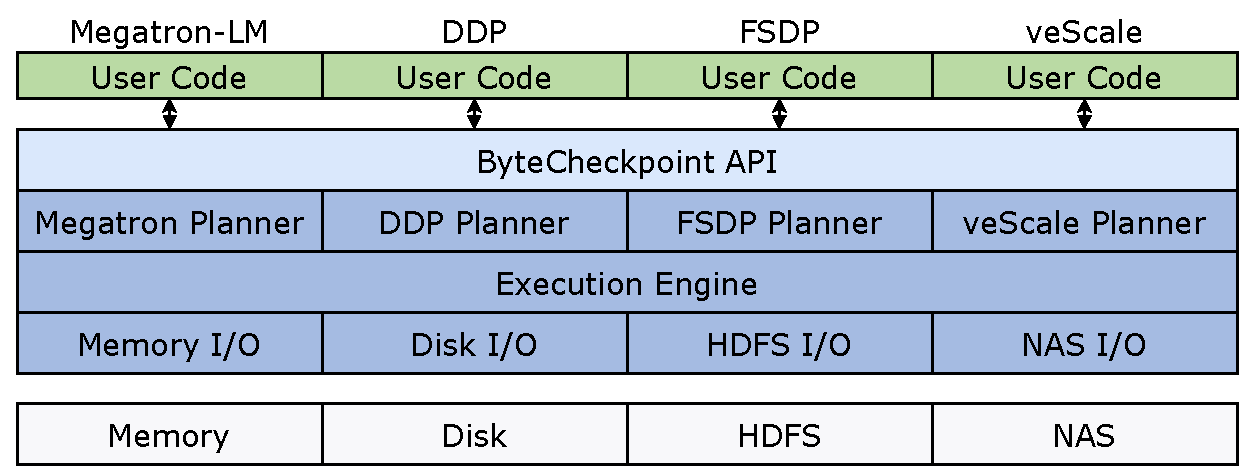
\includegraphics[width=\linewidth]{figures/architecture.pdf}
  \caption{Architecture of \sys{}. 
  % \cwu{arrows between I/O and respective storage backend are missing}
  }
  \label{fig:architecture}
\end{figure}

Based on the above observations, we design \sys{} according to the following key principles:

\noindent \textit{(1) Decoupling}.
The checkpoint representation remains independent of specific runtime parallelism.
Interfaces of training frameworks and storage backends are separated from the core execution engine, ensuring robust extensibility.

\noindent \textit{(2) User-friendliness}.
The APIs should be concise, making it seamless for AI researchers and engineers to integrate them into their code and runtime environments.
% We present \sys{}, a unified checkpointing system for LFM development that supports multiple training frameworks and storage backends.

\subsection{Unified Architecture}
\label{sec:arch}
%In the following sections, we provide a detailed discussion of each layer within this architecture.
The architecture of \sys{} is illustrated in Fig.~\ref{fig:architecture}.
Each component is introduced in detail as follows: 

\noindent \textbf{API.} \sys{}'s APIs (\texttt{bytecheckpoint.save} and \texttt{bytecheckpoint.load}) provide a unified entrypoint for user code across various training frameworks.
For instance, to save checkpoints, users first prepare the corresponding training states, checkpoint path, framework name, and performance-related options, then call \texttt{bytecheckpoint.save}.
% on each training worker.
% xx \cwu{give what the API exactly is}. % similar to PyTorch native API  like \texttt{torch.save()} and \texttt{torch.load()}, eliminating additional learning curves for users. 
% \cwu{tell how users use the APIs:} 
% \cwu{in each process on each GPU or what} 
% when xx for saving checkpoints to xx, providing a dictionary containing the relevant training states, checkpoint path, framework name, and performance optimization options.
% To load checkpoints, users prepare similar arguments and call \texttt{bytecheckpoint.load} 
% \cwu{in which process}
% in each training worker when loading saved checkpoints back to arbitrary parallelism. 
This high-level entrypoint abstracts underlying system complexities, such as sharding specification, save/reshard plan generation, and I/O operations.

% The API is compatible with numerous frameworks and storage backends and remains independent of the parallelism setting.

% The underlying system complexities—such as device mesh configurations, save/reshard plan generation, and I/O operations—are abstracted away from the user. Furthermore, the API is designed to be agnostic to specific training frameworks, parallelism strategies, and storage backends. Fig.~\ref{fig:code_examples} shows an API usage example.


\noindent \textbf{Planner.}
% \cwu{tell the connection/relation between API and planner}
The Planner serves as the interface for training frameworks.
It receives arguments (training states, checkpoint path, etc.) from the API layer, creates ShardMeta (Sec.~\ref{sec:represent}) for each tensor shard based on the worker's rank and framework-specific sharding specification such as \textit{Megatron ShardedTensor} or \textit{FSDP DTensor}, and determines the tensors and other states to save/load for each worker.
Each worker leverages the Planner to initially create local plans and subsequently collaborates to create global plans.
% Given the framework-specific specifications,
% such as distributed tensor abstractions and device mesh configurations,
We implement a tailored planner for each training framework to extract information from these specifications and generate plans.

% \cwu{tell if the planner is running with each GPU process to make the local saving/loading plans}.
% \cwu{clarify what is tailored in the planner}.
%The Planner mainly comprises two steps: one \textit{gathering} step and one \textit{scattering} step.
% It first identifies the items to be saved or loaded from the provided dictionary, constructs the BasicMeta and ShardMeta for saving, or retrieves the global metadata file for loading purposes.
%After that, the coordinator planner, located in the worker with rank 0, gathers BasicMeta and ShardMeta or the ShardtoByteMap from others and applies workload distribution algorithms (refer to Sec.~\ref{sec:io_optimization} for a detailed explanation of the saving/loading workload partitioning mechanism) to create save/load plans.
%These plans specify which tensor shards each worker will save, transfer (for merging irregular shards), or load.
% The finalized plans are scattered to each worker and then forwarded to the Execution Engine to carry out the actual I/O tasks.
%The saving workflow includes an additional gathering step to gather the ByteMeta constructed from the storage files upon the completion of I/O tasks and assemble collected metadata into the final global metadata file.

\noindent \textbf{Execution Engine}.
The Engine, running on each training worker, executes the saving/loading plans generated by the Planner when the respective API is called. It analyzes the given checkpoint path to determine the appropriate storage backend, then interacts with the Storage I/O layer to execute the actual I/O tasks specified in the plans.
% \cwu{tell if the engine is run on each GPU process}
% \cwu{when the respective API is called?}.
% During the saving process, the different phases associated with saving each tensor shard (outlined in Sec.~\ref{sec:background}) are executed separately in a fully asynchronous pipeline, while the P2P communications for tensor merging are conducted concurrently.
% After the serialization and dump phases, the BasicMeta and ByteMeta are retrieved and used to construct the final global metadata file.
% By default, the checkpoint-saving workloads are handled by separated I/O processes to move them from the critical path of training.
% For loading, each process retrieves data from storage files and employs advanced techniques such as the zero redundancy loading mechanism to reduce loading costs.
% The Engine incorporates a number of I/O performance optimization techniques (Sec.~\ref{sec:io_optimization}).

%\textcolor{blue}{Mingji: Change from "Core Layer" to "Execution Layer"}

\noindent \textbf{Storage I/O}.
Analogous to the design of the Planner layer, the Storage I/O layer encapsulates different storage backends and manages backend-specific read/write operations and optimizations. 
%(see Appendix~\ref{sec:io_parallel} for an example of HDFS optimization)
The interface between the Engine layer and the Storage I/O layer remains unified across different storage backends, facilitating the seamless integration of new storage backends.
\sys{} supports multiple storage options, including in-memory checkpoint storage~\cite{gemini-sys}, local disk storage, and remote storage systems.
% (e.g., HDFS and NAS).
% \cwu{explicitly tell the connection between execution engine and storage I/O, i.e., does the engine calls the I/O according to the storage plan?} \brwan{put the description to Engine layer.}
% The Storage layer manages read and write operations across diverse storage backends and implements backend-specific optimizations.
% This modular design \cwu{what the modular design is referring to, are you referring to one storage layer I/O interface for each storage backend?} facilitates seamless integration of new storage backends, by xx \cwu{tell how to integrate with new storage backend}, thereby reducing development overhead. %Importantly, any optimizations implemented in the Storage layer benefit users across all supported training frameworks.

\begin{figure}[!t]
  \centering
  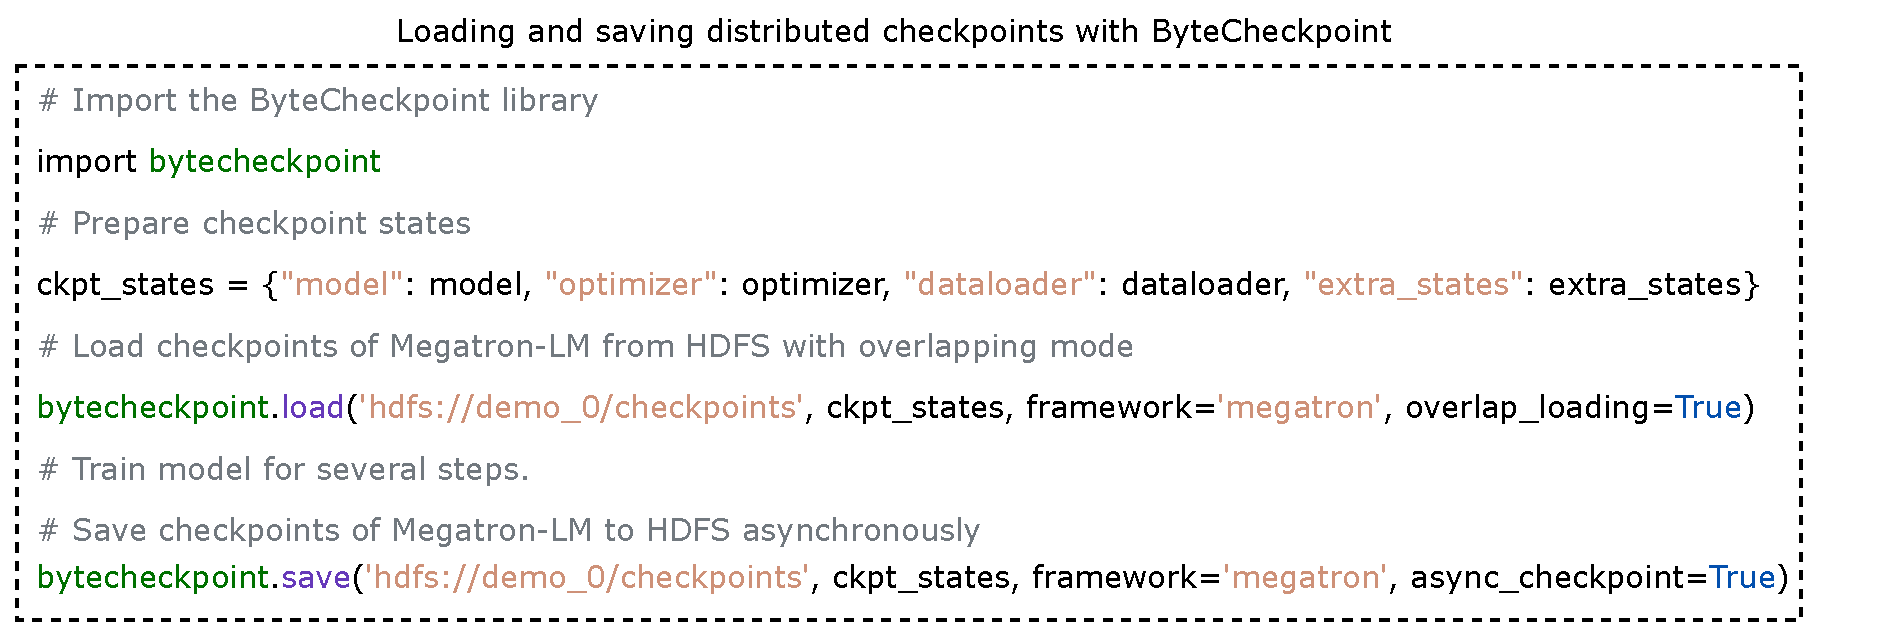
\includegraphics[width=\linewidth]{figures/code_examples.pdf}
  \caption{Examples of using \sys{}'s APIs.
  % \textcolor{blue}{Mingji: "parameter" -> "model" }
  }
  \label{fig:code_examples}
\end{figure}

Fig.~\ref{fig:code_examples} illustrates a typical use case of \sys{}. Initially, users define a dictionary specifying the states to be saved or loaded, encompassing the model, optimizer, dataloader, and additional states.
% Checkpoint operations are subsequently performed using \texttt{bytecheckpoint.save} and \texttt{bytecheckpoint.load} API calls.
At the outset of training resumption, stage transition, or evaluation, \texttt{bytecheckpoint.load} is invoked to load saved checkpoints.
Checkpoint resharding occurs automatically during loading when there are changes in parallelism.
During training, \texttt{bytecheckpoint.save} is periodically invoked to save checkpoints.
% \cwu{give concrete examples on how the APIs are called in training resumption, evaluation task and cross-state transition cases.}

\subsection{Decoupled Checkpoint Representation}\label{sec:represent}
\begin{comment}
\begin{figure}[!t]
  \centering
  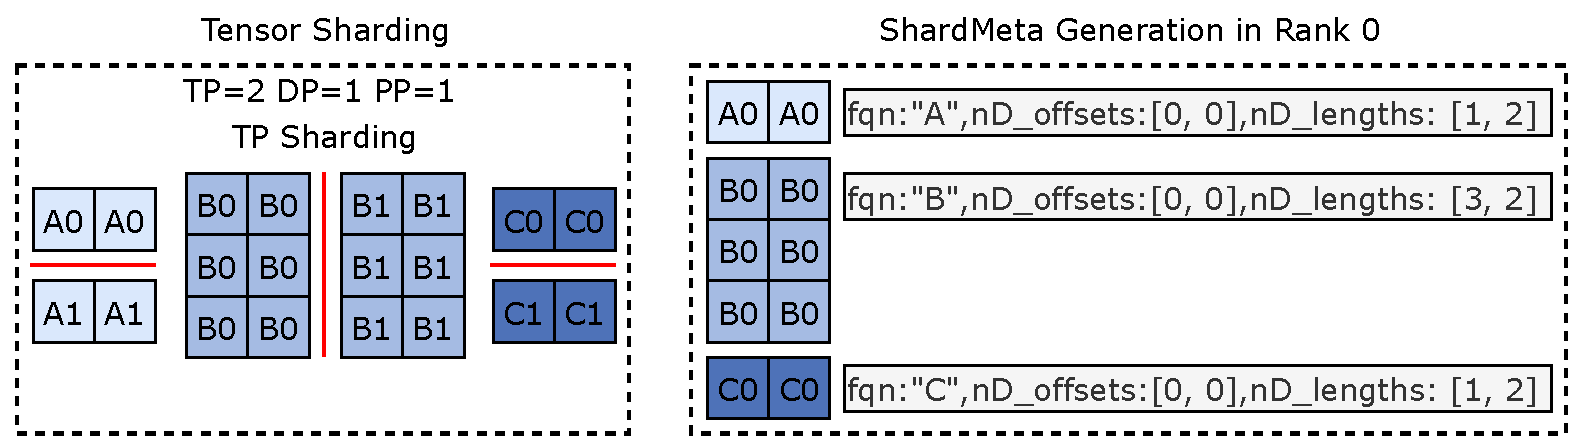
\includegraphics[width=\linewidth]{figures/regular_tensor.pdf}
  \caption{
  ShardMeta generation of tensor-parallel sharded tensors.
  }
  \label{fig:decomposed_meta}
\end{figure}    
\end{comment}

% Give an overview here.
% How a checkpoint can be represented.

%\noindent \textbf{Sharding spec.}
To achieve parallelism-agnostic checkpointing to enable automatic load-time resharding, we develop a formal specification of model and optimizer tensors in distributed training. Our design conforms to the Distributed Tensor and Checkpoint concepts in the \textit{PyTorch Distributed} library~\cite{ddp}.
% \cwu{add citation}

\noindent \textbf{Model and optimizer states.}
Each tensor is uniquely identified by a "fully qualified name" (FQN) and has a global shape, representing its original shape before sharding.
Tensors can be either sharded or replicated across ranks (aka training workers).
For sharded tensors, the specific shard held by a worker is determined by three factors: the parallelism (e.g., tensor parallelism) applied to the tensor, the sharding dimension, 
% (e.g., dimension 1 for an MLP weight tensor),
and the group rank within the corresponding parallelism group. Based on a tensor's FQN, global shape, and sharding specification, \sys{} creates the tensor shard metadata (ShardMeta) for each rank, which is utilized in checkpoint storage to represent the tensor shard, independent of parallelism.
More precisely, ShardMeta for a tensor shard is an index tuple \textit{(fqn, nD\_offsets, nD\_lengths)}, where \textit{nD\_offsets} and \textit{nD\_lengths} indicate the local shard's offsets and lengths along the original multi-dimensional axes in its global shape.
%multiple shards collectively form the complete tensor. 
%This rank information is obtained from DeviceMesh, a high-level abstraction that manages process groups.
% \cwu{the \textit{ShardMeta} is an?}
% \cwu{clarify what this global shape is referring to}.%In the case of replication, all processes share an identical copy of the tensor. 
% \cwu{explain}. % to facilitate a general representation of tensor shards. 
% In the example in Fig.~\ref{fig:decomposed_meta}, tensors A, B, and C are sharded on dimension 0 or 1, and %can be directly represented by 
% the index tuples to represent the tensor shards on rank 0 are depicted on the right side of the figure.
% \cwu{spell out the tuples as examples.} \cwu{no FQN in the tuples in the figure?}. 

\begin{figure}[!t]
  \centering
  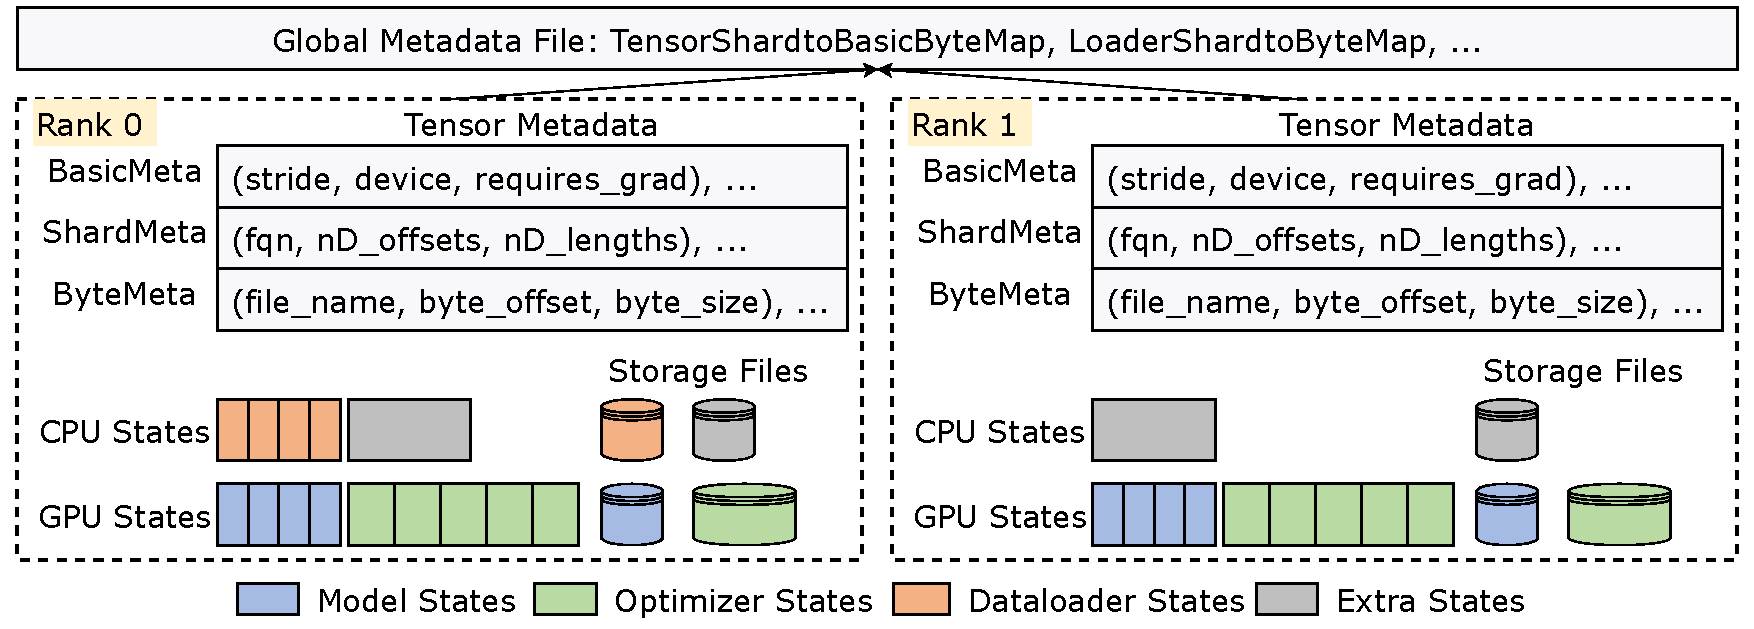
\includegraphics[width=\linewidth]{figures/representation.pdf}
  \caption{
  Checkpoint representation in \sys{}.
  The pipeline parallelism is applied in this example.
  % \cwu{Replicated?} 
  % Dataloader states are saved by rank 0.
  % whose group ranks, \cwu{`for all degrees of parallelism, except the DP degree' is just in the PP degree}, are 0. 
  }
  \vspace{-5mm}
  \label{fig:representation_meta}
\end{figure}

\noindent \textbf{Dataloader and extra states.}
%Dataloader states are categorized into \textit{replicated} and \textit{sharded} states.
%Sharded states are saved in individual files whereas replicated states are saved only by rank 0.
%Extra states are directly packed and dumped into storage.
%For more details, refer to Appendix~\ref{sec:loader_extra}.
The dataloader states can be categorized into two types: \textit{replicated} states and \textit{sharded} states. Replicated states include the number of data reading workers, paths to source datasets, and sampling ratios, and are identical across all I/O workers (subprocesses) in different ranks.
% \cwu{clarify what an I/O worker is}
Sharded states are unique to each I/O worker, including the token buffer %(as described in Sec. 2) 
and data retrieval offsets for different data sources. % Our system, \
In \sys{}, %employs an efficient storage strategy: 
sharded states are saved in individual files, while replicated states are saved only by the I/O worker in rank 0. This %approach offers two key advantages: 
reduces overall %checkpoint 
size of dataloader states to be saved and facilitates dataloader resharding when parallelism configurations change since the separation of data states into distinct files simplifies %the process of 
states merging and redistributing according to the new parallelism. For other extra states such as the RNG state, we pack and 
serialize them into one compact byte object before dumping them into storage.

\noindent \textbf{Checkpoint representation.}
Fig.~\ref{fig:representation_meta} illustrates the checkpoint representation in \sys{}.
Distributed checkpoints comprise a \textit{global metadata file}
and multiple \textit{storage files}.
Each rank 
% invokes \sys{} to 
generates three distinct files: a model state file, an optimizer state file, and an extra state file.
The Dataloader state file is generated only by training workers whose ranks for all parallelism degrees, except for DP degrees, are 0.
For tensor shards in model and optimizer states, their \textit{Metadata} consists of three parts:
\textit{BasicMeta}, which records essential information of individual tensor shards such as stride and device, critical for recovering the runtime state;
\textit{ShardMeta}, as previously introduced, recording relative position information of shards in the complete tensor;
\textit{ByteMeta}, which specifies the byte start offset and length of each tensor shard within the storage file.
All tensor metadata are consolidated into the global metadata file, and a mapping, termed \textit{TensorShardtoBasicByteMap}, is established between saved tensor shards and storage files based on the ShardMeta, BasicMeta, and ByteMeta of each tensor shard, ensuring accurate data retrieval.
The global metadata file also includes a \textit{LoaderShardtoByteMap}, which records the file index information of sharded states in each dataloader.
All storage files and the global metadata file are
stored in the specified storage backend designated by the checkpoint path.
% when \texttt{bytecheckpoint.save} is invoked.

\begin{figure}[!t]
  \centering
  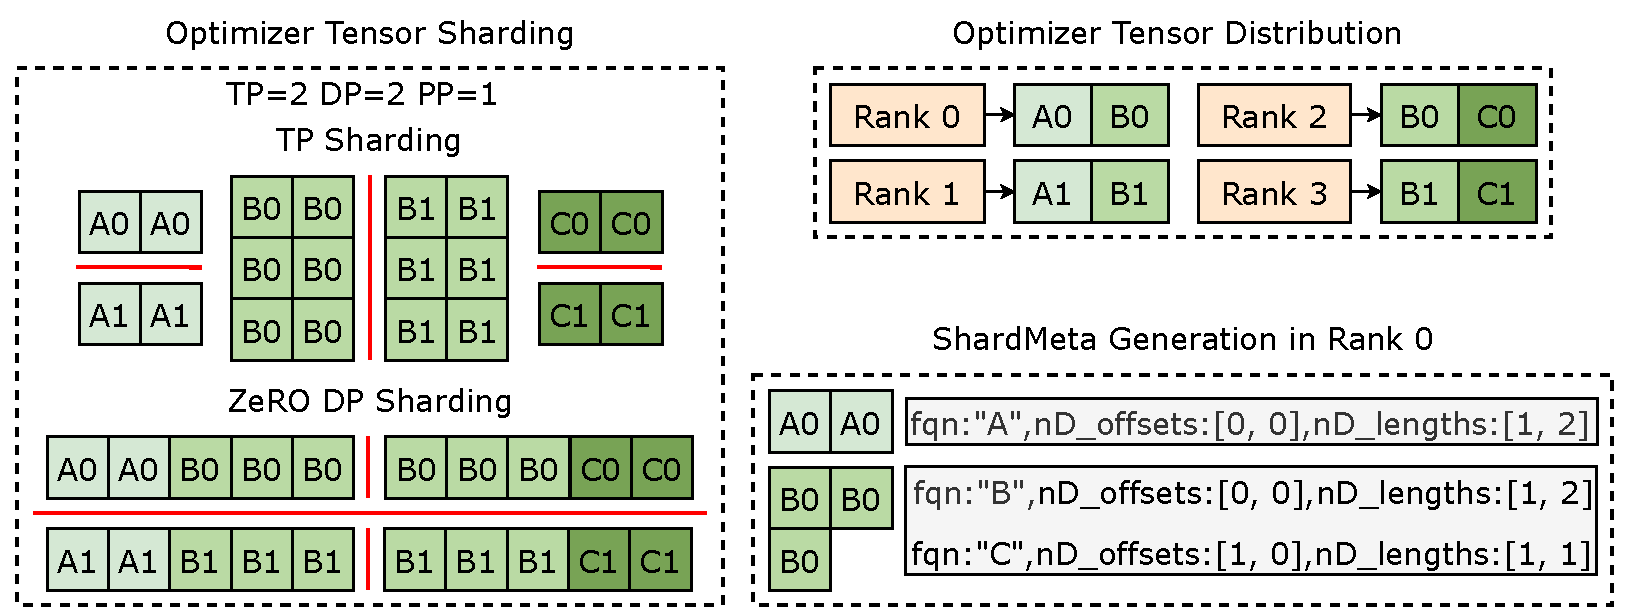
\includegraphics[width=\linewidth]{figures/irregular_tensor.pdf}
  \caption{
  ShardMeta of irregular tensors in optimizer states.
  }
  \label{fig:irregular_decomposed_meta}
  \vspace{-5mm}
\end{figure}
% \yhpeng{The sentences and paragraphs in this subsection need to be reorganized. First, introduce what is irregular tensor, why it exists, and whether Megatron-LM and PyTorch support it; Second, what is the naive way to save irregular tensor and what is the overhead (introduce tensor merging solution); Third, describe how we handle irregular tensor effciciently.}

\noindent \textbf{Decomposing irregular tensors}.
We define irregular tensors as those which, when flattened before sharding, cannot be reshaped back to their original dimensions. These tensors typically arise when applying the Zero Redundancy Optimizer (ZeRO)\cite{zero}, as implemented in Megatron-LM ZeRO2 and FSDP ZeRO3\cite{fsdp}. In these implementations, optimizer states within a DP group are flattened, concatenated, and sharded. Consequently, the resulting 1D tensor slices often cannot be directly represented using n-dimensional shapes and offsets.
Fig.~\ref{fig:irregular_decomposed_meta} illustrates an example of irregular tensor sharding: Unlike tensors $A$ and $C$, tensor $B$, with an original shape of (3, 2), is evenly split into two shards. Each shard, containing three elements, cannot be directly represented as a two-dimensional shape with corresponding offsets.
One intuitive approach to addressing the challenge of irregular tensor shards is to merge all tensor shards into complete tensors before saving checkpoints, thereby simplifying the generation of ShardMeta.
For example, to eliminate potential irregular tensors in DCP~\cite{torch-dcp}, FSDP performs synchronous all-gather communication operations, interleaved with D2H copy operations for each tensor shard, regardless of whether the shard is irregularly sharded.
However, this approach incurs significant communication overhead and requires frequent synchronization between GPU and CPU, substantially impeding efficiency.

To mitigate the overhead associated with merging tensor shards, \sys{} employs a tensor decomposition strategy for managing irregular tensor shards. Specifically, \sys{} decomposes an irregular tensor into a series of regular ones, representing each with index tuples. For example, consider the irregular tensor shard of tensor $B$ with three elements on rank $0$ in Fig.~\ref{fig:irregular_decomposed_meta}. \sys{} decomposes this shard into two regular tensors that can be directly represented by $nD\_offsets$ and $nD\_lengths$. This approach allows \sys{} to use multiple \textit{ShardMeta} entries to represent a single irregular tensor shard.
Although such decomposition slightly increases the metadata size and adds steps to the loading procedure, as reconstructing the target tensor may require looking up multiple smaller segments of irregular shards, it avoids the costly communication of tensor shards without extra blocking time during saving.

\subsection{Checkpoint Resharding %Generic
Workflow}

\label{sec:workflow}

% How to achieve resharding.
\begin{figure}[!t]
  \centering
  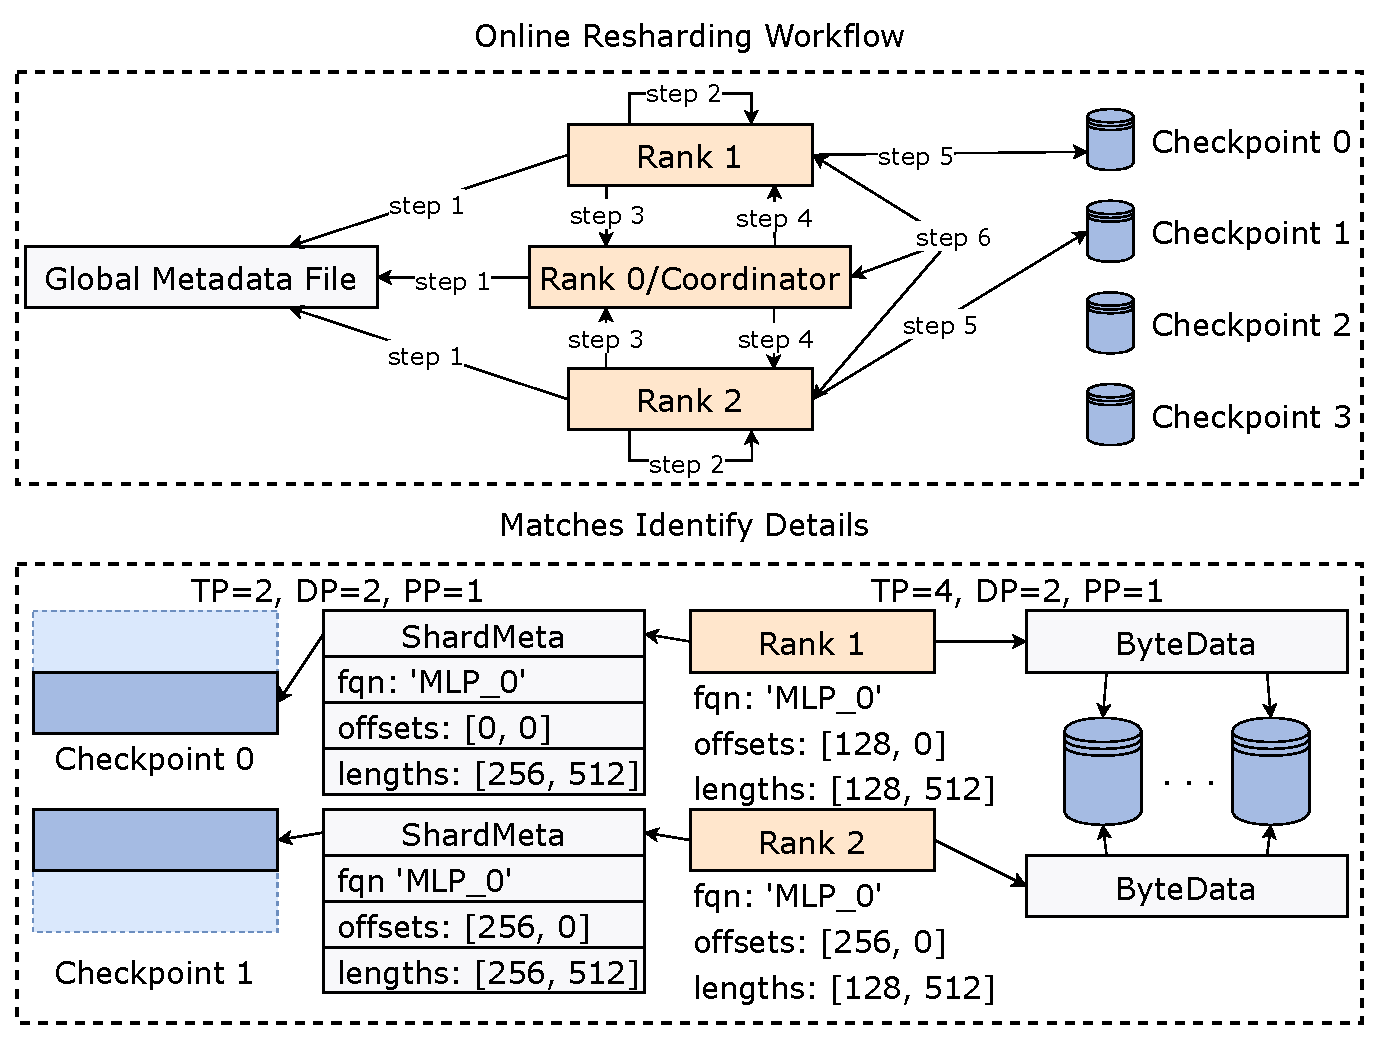
\includegraphics[width=\linewidth]{figures/tensor_reshard_examples.pdf}
  % \includegraphics[width=\linewidth]
  % {figures/tensor_reshard_examples2.pdf}
  \caption{
  Load-time tensor resharding workflow.
  % Assume that each tensor shard is retained in its original shape before saving.
  Checkpoint $k$ denotes the checkpoint saved by a previous live worker $k$.
  % The distributed checkpoints are saved with parallelism configuration: TP=2, DP=2 PP=1, and are loaded into configuration: TP=4, DP=2, PP=1.
  % To provide a comprehensive view, we show processes with rank 1 and 2 for model states resharding while rank 0 and 15 for optimizer states resharding.
  % PP resharding can also be naturally supported by looking up FQN in ShardMeta to load target tensor shards. 
  % \zmf{add labels of original ranks in the above fig to indicate from which rank the ckpt files are saved of the 3d parallelism configuration before resharding?}
  }
  \vspace{-5mm}
  \label{fig:tensor_reshard_example}
\end{figure}
% 
% Overview of the system. 
% The workflow of \sys{} is illustrated in Fig.~\ref{fig:architecture}.
%\sys{} offers a unified interface that accommodates various training frameworks and facilitates interactions with a range of storage backends, including Cloud File System (CFS), local disks, HDFS, and NAS.
%By decoupling the Planner Layer and the Storage Layer from the Execution Layer, \sys{}'s extensibility is significantly enhanced.
\sys{} implements a generic workflow for saving and loading, automatically resharding checkpoints during the loading process. Leveraging the independence between the Engine Layer, Planner Layer, and Storage I/O Layer, we can execute consistent saving and loading steps across different training frameworks and storage backends. We take tensor resharding as an example
% to illustrate the checkpoint resharding workflow below and
in Fig.~\ref{fig:tensor_reshard_example}, emphasizing how our checkpoint representation enables flexible load-time resharding.
% for GPU states.
The process for checkpoint saving and loading without resharding follows a similar procedure.

\noindent \textbf{Step 1}.
To initiate load-time checkpoint resharding, each rank invokes the \texttt{bytecheckpoint.load()} API, specifying the checkpoint path along with the model/optimizer
% dataloader, and extra states
to be restored.
All ranks then load the global metadata file from the 
% designated checkpoint
path.

\noindent \textbf{Step 2}.
For each tensor shard in the given model/optimizer, each rank queries the TensorShardToBasicByteMap within the global metadata file, identifying matching segments between the saved tensor shards and the sharding specification of new shards.
After identifying these matches, the planner constructs a local load plan, which includes BasicMeta and ByteMeta tailored to the specific shard. This identification mechanism is illustrated at the bottom of Fig.~\ref{fig:tensor_reshard_example}.

\noindent \textbf{Step 3}.
The coordinator planner, typically residing in rank 0, initiates a gather operation to aggregate loading plans from all ranks. It then optimizes each local plan by applying the redundant elimination optimization (Sec.~\ref{sec:opt_plan}) to distribute tensor shard loading workloads for reduced completion time.

\noindent \textbf{Step 4}.
The coordinator initiates a scatter operation to distribute the finalized loading plan. Each rank then receives its final loading plan from the coordinator.

\noindent \textbf{Step 5}.
The execution engine on each rank selects the storage backend wrapper in the Storage I/O layer based on the checkpoint path and then executes the loading pipeline (Sec.~\ref{sec:opt_pipeline}).

\noindent \textbf{Step 6}.
Upon completion of the loading pipeline, each rank utilizes the optimized asynchronous collective barrier primitive ensuring the atomicity of the distributed loading. Further details can be found in Appendix~\ref{sec:barrier_check}.

\noindent \textbf{Dataloader resharding}.
Similar to tensor resharding in Fig~\ref{fig:tensor_reshard_example}, \sys{} reshards the dataloader by querying the LoaderShardtoByteMap.
% \yhpeng{we need to find a better place to discuss dataloader resharding.}
The illustration of dataloader resharding is depicted in Fig.~\ref{fig:loader_reshard_example}. When parallelism configuration changes, for the dataloader checkpoints, common items in the dataloader checkpoints can be loaded directly, whereas unique items such as accumulative token buffers and data retrieval offsets require resharding. Specifically, when the DP degree size remains constant while other parallel degrees are altered (TP degree changes in the example of Fig.~\ref{fig:loader_reshard_example}), the token buffers should be copied to the destination workers for bitwise-correct resuming. when there is a change in the DP degree size, the token buffers must be either split or merged accordingly to ensure that the resumed dataloaders do not discard cached data and do not retrain data that has already been sampled and fed. Thanks to the split storage strategy designed for the dataloader module, \sys{} can precisely identify the unique items that require resharding and process them efficiently.

\begin{figure}[!t]
  \centering
  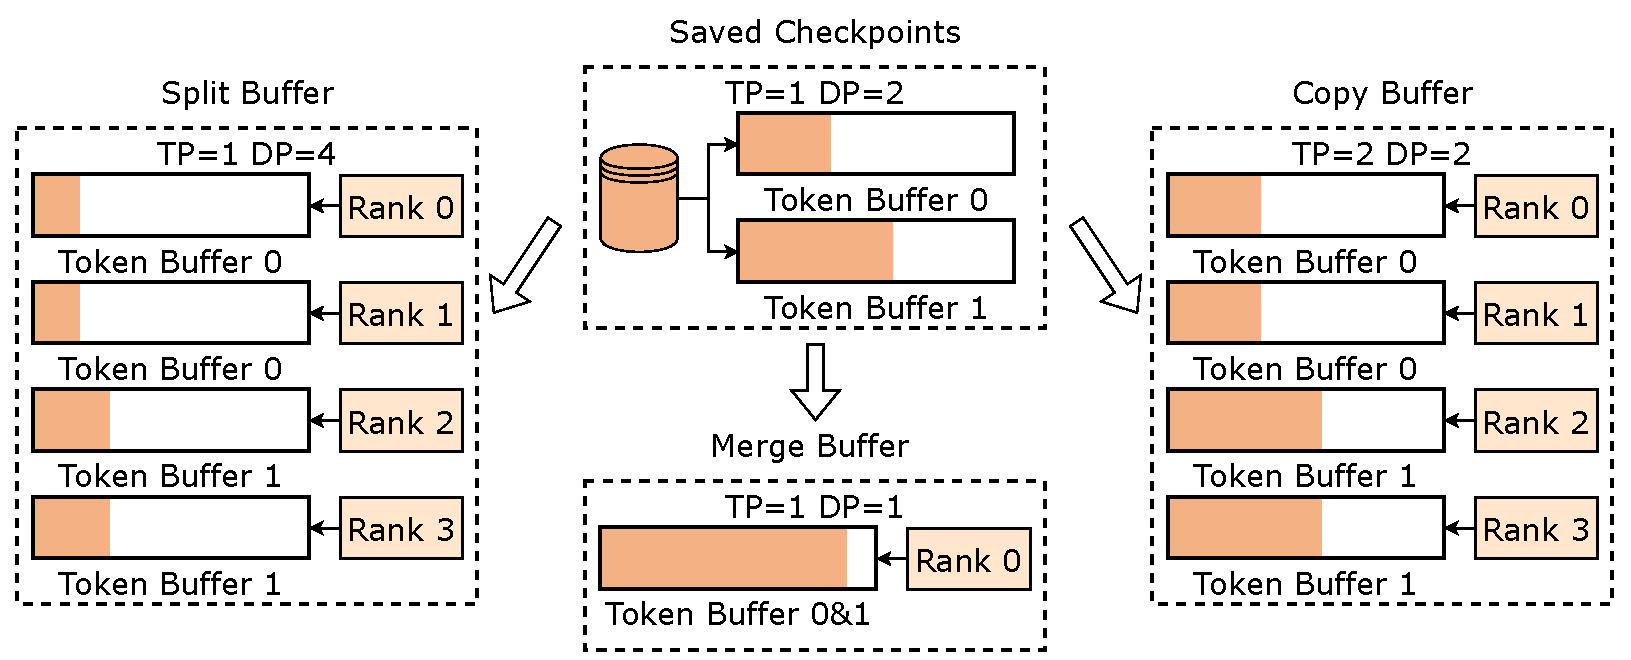
\includegraphics[width=\linewidth]{figures/loader_reshard_examples.pdf}
  \caption{
  Examples of dataloader resharding.
  Sharded states such as cumulative token buffers are resharded according to the changes of 
  parallelism configurations.
  We do not depict data retrieval offsets for clarity of the figure.
  }
  \label{fig:loader_reshard_example}
\end{figure}

%\sys{} also supports dataloader state resharding, which merges, splits, or copies token buffers as parallelism changes.
%For more information, see Appendix~\ref{sec:dataloader_reshard}.
%implements the loading plan to retrieve tensor shards from the file system \cwu{clarify what file system this is referring to, the storage backend?}.
% It leverages an appropriate I/O component (HDFS or Disk I/O) based on the filesystem type associated with the checkpoint path.

%\noindent \textbf{Step 6}. Communication between ranks would be involved afterwards %in the sixth step
% if replicated tensor loading is replaced by broadcast.
% After that, BasicMeta is utilized to recover the final runtime states of the target tensor shard.
% which is not depicted in Fig.~\ref{fig:reshard_example} for clarity.

% This entire procedure runs automatically when \texttt{bytecheckpoint.load()} is invoked, without requiring explicit specification of the loaded checkpoint's parallelism settings \cwu{not clear in which step above, loaded checkpoint's parallelism is fulfilled}.

%\noindent \textbf{Saving and Loading Workflow}. When save/loading API is called, planner creates saving/loading plan. The planning mainly comprises two steps: one \textit{gathering} step and one \textit{scattering} step.
%Each process first identifies the items to be saved or loaded from the provided dictionary, constructs the BasicMeta and ShardMeta for saving, or retrieves the global metadata file for loading purposes. After that, the coordinator planner, located in the worker with rank 0, gathers BasicMeta and ShardMeta or the ShardtoByteMap from others and applies workload distribution algorithms (refer to Sec.~\ref{sec:io_optimization} for a detailed explanation of the saving/loading workload partitioning mechanism) to create save/load plans.
%These plans specify which tensor shards each process will save, transfer (for merging irregular shards), or load.
%The finalized plans are scattered to each process and then forwarded to the Execution Engine to carry out the actual I/O tasks. 

% During the saving process, the different phases associated with saving each tensor shard (outlined in Sec.~\ref{sec:background}) are executed separately in a fully asynchronous pipeline, while the P2P communications for tensor merging are conducted concurrently.
% After the serialization and dump phases, the BasicMeta and ByteMeta are retrieved and used to construct the final global metadata file.
% By default, the checkpoint-saving workloads are handled by separated I/O processes to move them from the critical path of training.
% For loading, each process retrieves data from storage files and employs advanced techniques such as the zero redundancy loading mechanism to reduce loading costs.
%The saving workflow includes an additional gathering step to gather the ByteMeta constructed from the storage files upon the completion of I/O tasks and assemble collected metadata into the final global metadata file. 

% When saving a checkpoint, it starts by copying tensors from the device to the host, then begins I/O operations to serialize and write the tensors to local SSDs or shared memory. If the checkpoint destination is on a remote storage system like HDFS or NFS, it uses a backend thread to upload the checkpoint asynchronously. When loading a checkpoint, it reads the tensors based on the loading plan and the metadata of the current checkpoint. 



